\documentclass[a4paper,12pt]{article}
\usepackage{ucs}
\usepackage[utf8x]{inputenc}
\usepackage{amsfonts}
\usepackage[english,russian]{babel}
\usepackage[T1,T2A]{fontenc}
\frenchspacing
\usepackage{amsmath,amssymb,amsthm}
\usepackage[a4paper, margin=1in]{geometry}
\usepackage[table]{xcolor}
\usepackage{multirow}
\usepackage{diagbox}
\usepackage{graphicx}
\graphicspath{ {./} }

\newtheorem{name}{Printed output}
\newtheorem{problem}{Задача}
\newenvironment{solution}{\renewcommand{\proofname}{\unskip\indent\nopunct}\begin{proof}}{\end{proof}}

\begin{document}

\title{ДЗ 4}
\author{Витя\,Ефремов}
\maketitle

\begin{problem}
Студент сдает 3 экзамена: математику, физику и информатику.
Вероятность успешно сдать математику 60\%, физику – 30\%, информатику – 80\%.
Пусть случайная величина X – количество сданных экзаменов.
Найти её закон распределения, функцию распределения, математическое ожидание, дисперсию.
\end{problem}
\begin{solution}
Всего три экзамена, поэтому случайная величина принимает значения от 0 до 3.
Закон распределения.
\begin{align*}
& P(X=0) = 0.4 \cdot 0.7 \cdot 0.2 & = 0.056 \\
& P(X=1) = 0.6 \cdot 0.7 \cdot 0.2 +  0.4 \cdot 0.3 \cdot 0.2 + 0.4 \cdot 0.7 \cdot 0.8 & = 0.332 \\
& P(X=2) = 0.4 \cdot 0.3 \cdot 0.8 + 0.6 \cdot 0.7 \cdot 0.8 + 0.6 \cdot 0.3 \cdot 0.2 & = 0.468 \\
& P(X=3) = 0.6 \cdot 0.3 \cdot 0.8 & = 0.144
\end{align*}

Функция распределения -- это просто кумулятивная сумма вероятностей.
Её график:

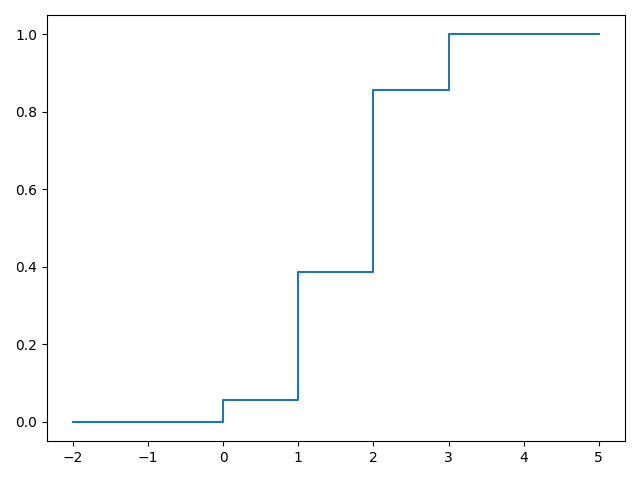
\includegraphics[width=\textwidth]{hw_4.1}

Матожидание:
$$\mathbb E[X] = \sum_{i = 0}^{3} P(X=i) \cdot i = 0.056 \cdot 0 + 0.332 \cdot 1 + 0.468 \cdot 2 + 0.144 \cdot 3 = 1.7$$

Дисперсия:
\begin{align*}
D[X] = \mathbb E[X^2] - (\mathbb E[X])^2 = \sum_{i = 0}^{3} P(X=i) \cdot i^2 - (\mathbb E[X])^2 & = \\
0.056 \cdot 0^2 + 0.332 \cdot 1^2 + 0.468 \cdot 2^2 + 0.144 \cdot 3^2 - 1.7^2 & = 0.61
\end{align*}
\end{solution}
\end{document}
